\documentclass[../part_1.tex]{subfiles}

\begin{document}
    \subsubsection{DINO}

    \par Интуитивно кажется что решение задачи \acrshort{mlm} не способствует тому что модель будте понимать структуру кода или какие-либо отличительные черты. 
    \par В ходе исследования внимание было обращено внимание на метод обучения \acrshort{dino}\cite{caron2021emergingpropertiesselfsupervisedvision} разработанный FacebookResearch. Он позволяет эффективно обучать модели на изображениях без разметки, извлекая универсальные визуальные представления. 
    \par Ключевая идея \acrshort{dino} — обучение через "самодистилляцию", когда модель учится согласовывать разные измененные версии одного изображения, не требуя предварительно размеченных данных.
    \par Для обучения исопльзуется две модели -- учитель и ученик. Учитель генерирует эталонные представления изображения, тогда как ученик пытается предсказать выход учителя. 
    \par В процессе обучения изображения разделяются на участки. Сначала из изображения выделяются два глобальных участка(изображение включающее 90\% исходного). Затем из изображения выделяются шесть локальных участков (изображения включающие около 15\% исходного). После этого к каждому набору учатско применяются аугментации(например отражение, изменене цветов и так далее) и глобальные участи передаются в учителя, а локальные в ученика.
    \begin{figure}[h]
        \centering
        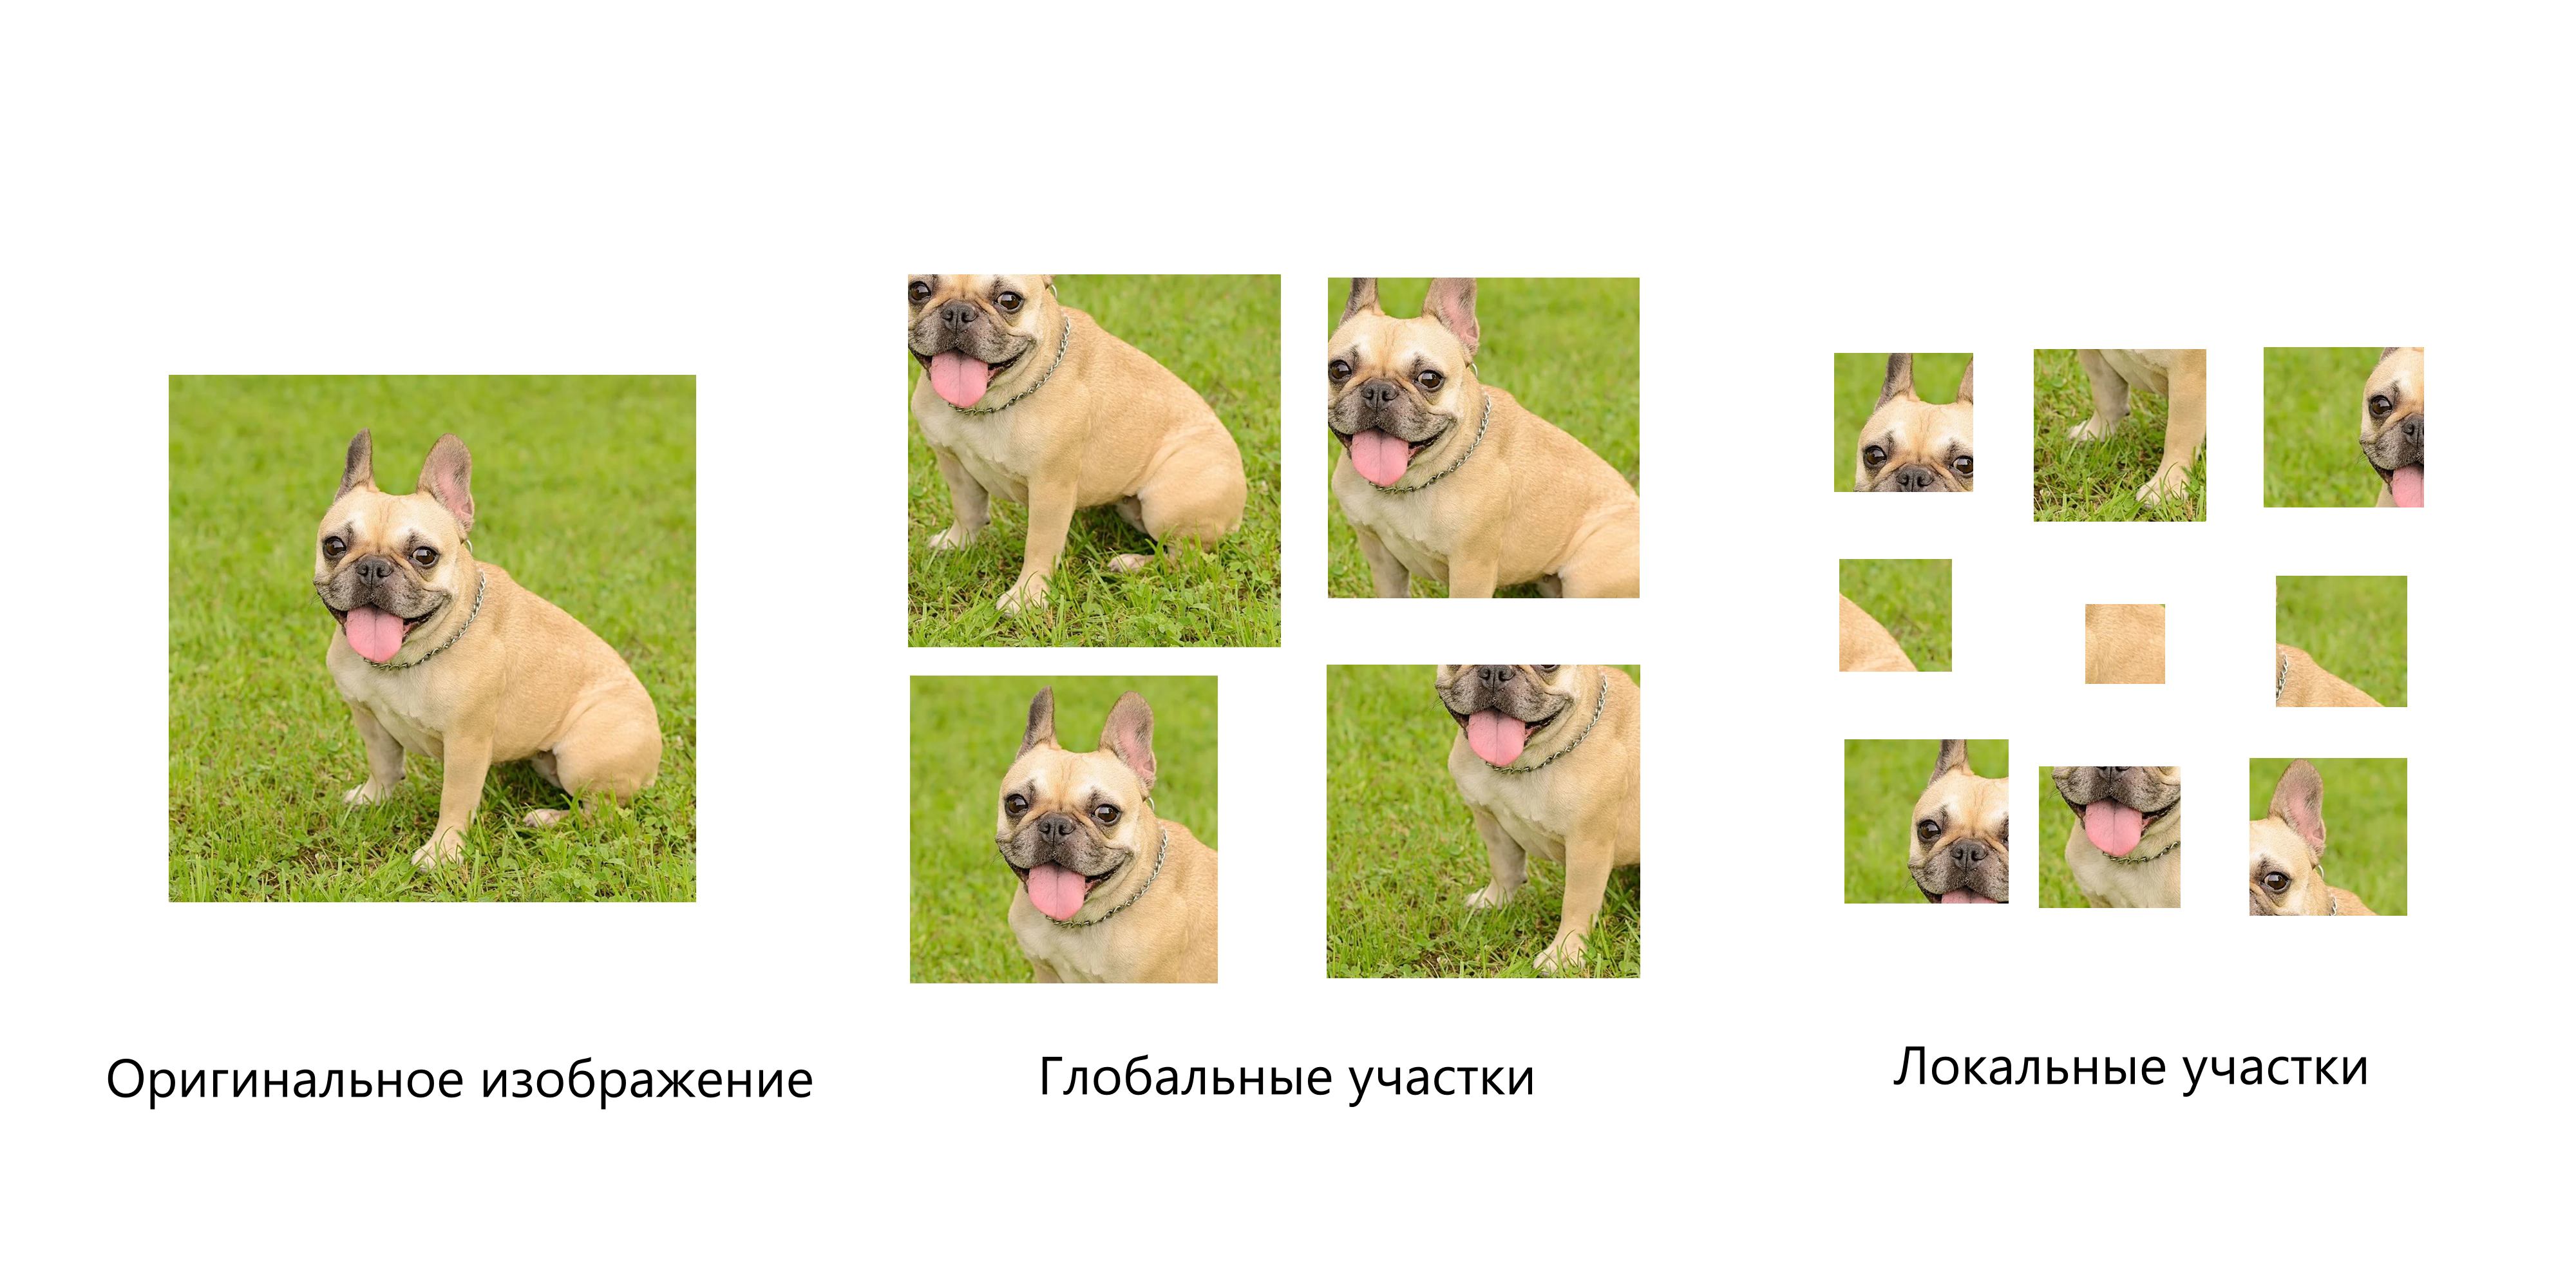
\includegraphics[width=0.6\textwidth]{multicrop_augment.png}
        \caption{Пример multicrop augmentation}
        \label{fig:multicrop_augment}
    \end{figure}
    \par Так же в loss функции используется техника заострения(Sharpening), которая делает выходное вероятностное распределениие более пиковым, уменьшая энтропию и подчеркивая наиболее вероятные классы. Это помогает избежать тривиальных решений, когда модель вырождается  и предсказывает равномерное распределение для всех входов. Sharpening выглядит как Softmax с параметром $\tau$.
    \begin{equation}
        \label{sharpening}
        P(x)^{(i)} = \frac{exp\Big(\frac{g_\theta(x)^{(i)}}{\tau}\Big)}{\Sigma^K_{k=1}exp\Big(\frac{g_\theta(x)^{(k)}}{\tau}\Big)}
    \end{equation}
    \par В формуле \ref{sharpening} показана функция sharpening для $i$ элемента модели $g$ с параметрами $\theta$. 
    \begin{equation}
        \label{cross_entropy}
        Loss = -P_t(x) \log \P_s(x)
    \end{equation}
    \par В формуле \ref{cross_entropy} показана функция потерь для учителя и студента.
    \par В качестве Loss функции используется стандартная кросс этнтропия.
    \par В процессе обучения ученик изменяет свои веса таким образом чтобы уменьшить разницу предсказания с предсказанием учителя. Веса учителя постепенно изменяются обновбляясь как экспоненциальное скользящее среднее весов ученика.
    
\end{document}